\documentclass{article}

\usepackage[margin=1em]{geometry}
\usepackage{subcaption}
\usepackage{tikz}

\usepackage{amsmath, amssymb}
\DeclareMathAlphabet{\mathpzc}{OT1}{pzc}{m}{it}

\title{Algebra of color shufflings for cube faces}
\date{}

\def\vspacing{50pt}
\tikzstyle{shuffle}=[shorten <= 5pt , shorten >= 5pt, line width = 1.5pt, line cap=round]
\tikzstyle{omitted}=[lightgray, dashed]

\begin{document}
	\maketitle

	\section{Generators}
	\begin{figure}[h!]
		% Element xyz
		\begin{subfigure}{0.24\textwidth}
			\centering
			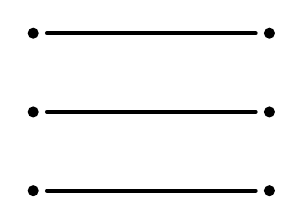
\begin{tikzpicture}
				\coordinate (xl) at (0,2);
				\coordinate (yl) at (0,1);
				\coordinate (zl) at (0,0);
				\coordinate (xr) at (3,2);
				\coordinate (yr) at (3,1);
				\coordinate (zr) at (3,0);

				\fill[black] (xl) circle [radius=2pt];
				\fill[black] (yl) circle [radius=2pt];
				\fill[black] (zl) circle [radius=2pt];

				\fill[black] (xr) circle [radius=2pt];
				\fill[black] (yr) circle [radius=2pt];
				\fill[black] (zr) circle [radius=2pt];

				\draw[shuffle] (xl) -- (xr);
				\draw[shuffle] (yl) -- (yr);
				\draw[shuffle] (zl) -- (zr);
			\end{tikzpicture}
			\caption{Element {\tt xyz}}
		\end{subfigure}
		% Element oyz
		\begin{subfigure}{0.24\textwidth}
			\centering
			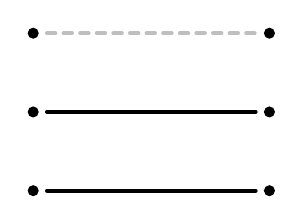
\begin{tikzpicture}
				\coordinate (xl) at (0,2);
				\coordinate (yl) at (0,1);
				\coordinate (zl) at (0,0);
				\coordinate (xr) at (3,2);
				\coordinate (yr) at (3,1);
				\coordinate (zr) at (3,0);

				\fill[black] (xl) circle [radius=2pt];
				\fill[black] (yl) circle [radius=2pt];
				\fill[black] (zl) circle [radius=2pt];

				\fill[black] (xr) circle [radius=2pt];
				\fill[black] (yr) circle [radius=2pt];
				\fill[black] (zr) circle [radius=2pt];

				\draw[shuffle, omitted] (xl) -- (xr);
				\draw[shuffle] (yl) -- (yr);
				\draw[shuffle] (zl) -- (zr);
			\end{tikzpicture}
			\caption{Element {\tt oyz}}
		\end{subfigure}
		% Element xoz
		\begin{subfigure}{0.24\textwidth}
			\centering
			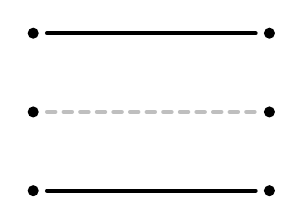
\begin{tikzpicture}
				\coordinate (xl) at (0,2);
				\coordinate (yl) at (0,1);
				\coordinate (zl) at (0,0);
				\coordinate (xr) at (3,2);
				\coordinate (yr) at (3,1);
				\coordinate (zr) at (3,0);

				\fill[black] (xl) circle [radius=2pt];
				\fill[black] (yl) circle [radius=2pt];
				\fill[black] (zl) circle [radius=2pt];

				\fill[black] (xr) circle [radius=2pt];
				\fill[black] (yr) circle [radius=2pt];
				\fill[black] (zr) circle [radius=2pt];

				\draw[shuffle] (xl) -- (xr);
				\draw[shuffle, omitted] (yl) -- (yr);
				\draw[shuffle] (zl) -- (zr);
			\end{tikzpicture}
			\caption{Element {\tt xoz}}
		\end{subfigure}
		% Element xyo
		\begin{subfigure}{0.24\textwidth}
			\centering
			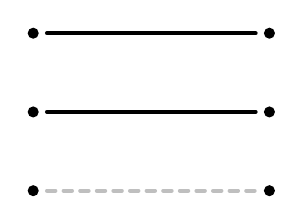
\begin{tikzpicture}
				\coordinate (xl) at (0,2);
				\coordinate (yl) at (0,1);
				\coordinate (zl) at (0,0);
				\coordinate (xr) at (3,2);
				\coordinate (yr) at (3,1);
				\coordinate (zr) at (3,0);

				\fill[black] (xl) circle [radius=2pt];
				\fill[black] (yl) circle [radius=2pt];
				\fill[black] (zl) circle [radius=2pt];

				\fill[black] (xr) circle [radius=2pt];
				\fill[black] (yr) circle [radius=2pt];
				\fill[black] (zr) circle [radius=2pt];

				\draw[shuffle] (xl) -- (xr);
				\draw[shuffle] (yl) -- (yr);
				\draw[shuffle, omitted] (zl) -- (zr);
			\end{tikzpicture}
			\caption{Element {\tt xyo}}
		\end{subfigure}
	\end{figure}

	\section{Extension operator $\otimes$}

	\begin{equation}
		(l_1l_2l_3, m) \otimes (r_1r_2r_3, n) = (u_1u_2u_3, m + n)
		\qquad\mbox{where}\qquad
		m, n \in \mathbb{N}
		\qquad\mbox{and}\qquad
		u_i ~=~ \begin{cases}
 			~~ \hfil {\tt o} & \mbox{if} ~ l_i = {\tt o} \\
 			~~ \hfil r_j & \mbox{if} ~ r_i = {\tt o} \wedge l_j = {\tt o} \\
 			~~ \hfil r_i & \mbox{if} ~ l_i \neq {\tt o} \neq r_i
		\end{cases}
	\end{equation}

	\begin{itemize}
		\item[$\hookrightarrow$] has identity {\tt xyz} but is \underline{not} associative	
	\end{itemize}


	\section{Path weights}
	
	\begin{equation}
		\mathpzc{CF} ~=~ \left( \mathbb{N}\right)
	\end{equation}


\end{document}